% Options for packages loaded elsewhere
\PassOptionsToPackage{unicode}{hyperref}
\PassOptionsToPackage{hyphens}{url}
\PassOptionsToPackage{dvipsnames,svgnames,x11names}{xcolor}
%
\documentclass[
  letterpaper,
  DIV=11,
  numbers=noendperiod]{scrartcl}

\usepackage{amsmath,amssymb}
\usepackage{iftex}
\ifPDFTeX
  \usepackage[T1]{fontenc}
  \usepackage[utf8]{inputenc}
  \usepackage{textcomp} % provide euro and other symbols
\else % if luatex or xetex
  \usepackage{unicode-math}
  \defaultfontfeatures{Scale=MatchLowercase}
  \defaultfontfeatures[\rmfamily]{Ligatures=TeX,Scale=1}
\fi
\usepackage{lmodern}
\ifPDFTeX\else  
    % xetex/luatex font selection
\fi
% Use upquote if available, for straight quotes in verbatim environments
\IfFileExists{upquote.sty}{\usepackage{upquote}}{}
\IfFileExists{microtype.sty}{% use microtype if available
  \usepackage[]{microtype}
  \UseMicrotypeSet[protrusion]{basicmath} % disable protrusion for tt fonts
}{}
\makeatletter
\@ifundefined{KOMAClassName}{% if non-KOMA class
  \IfFileExists{parskip.sty}{%
    \usepackage{parskip}
  }{% else
    \setlength{\parindent}{0pt}
    \setlength{\parskip}{6pt plus 2pt minus 1pt}}
}{% if KOMA class
  \KOMAoptions{parskip=half}}
\makeatother
\usepackage{xcolor}
\setlength{\emergencystretch}{3em} % prevent overfull lines
\setcounter{secnumdepth}{-\maxdimen} % remove section numbering
% Make \paragraph and \subparagraph free-standing
\makeatletter
\ifx\paragraph\undefined\else
  \let\oldparagraph\paragraph
  \renewcommand{\paragraph}{
    \@ifstar
      \xxxParagraphStar
      \xxxParagraphNoStar
  }
  \newcommand{\xxxParagraphStar}[1]{\oldparagraph*{#1}\mbox{}}
  \newcommand{\xxxParagraphNoStar}[1]{\oldparagraph{#1}\mbox{}}
\fi
\ifx\subparagraph\undefined\else
  \let\oldsubparagraph\subparagraph
  \renewcommand{\subparagraph}{
    \@ifstar
      \xxxSubParagraphStar
      \xxxSubParagraphNoStar
  }
  \newcommand{\xxxSubParagraphStar}[1]{\oldsubparagraph*{#1}\mbox{}}
  \newcommand{\xxxSubParagraphNoStar}[1]{\oldsubparagraph{#1}\mbox{}}
\fi
\makeatother

\usepackage{color}
\usepackage{fancyvrb}
\newcommand{\VerbBar}{|}
\newcommand{\VERB}{\Verb[commandchars=\\\{\}]}
\DefineVerbatimEnvironment{Highlighting}{Verbatim}{commandchars=\\\{\}}
% Add ',fontsize=\small' for more characters per line
\usepackage{framed}
\definecolor{shadecolor}{RGB}{241,243,245}
\newenvironment{Shaded}{\begin{snugshade}}{\end{snugshade}}
\newcommand{\AlertTok}[1]{\textcolor[rgb]{0.68,0.00,0.00}{#1}}
\newcommand{\AnnotationTok}[1]{\textcolor[rgb]{0.37,0.37,0.37}{#1}}
\newcommand{\AttributeTok}[1]{\textcolor[rgb]{0.40,0.45,0.13}{#1}}
\newcommand{\BaseNTok}[1]{\textcolor[rgb]{0.68,0.00,0.00}{#1}}
\newcommand{\BuiltInTok}[1]{\textcolor[rgb]{0.00,0.23,0.31}{#1}}
\newcommand{\CharTok}[1]{\textcolor[rgb]{0.13,0.47,0.30}{#1}}
\newcommand{\CommentTok}[1]{\textcolor[rgb]{0.37,0.37,0.37}{#1}}
\newcommand{\CommentVarTok}[1]{\textcolor[rgb]{0.37,0.37,0.37}{\textit{#1}}}
\newcommand{\ConstantTok}[1]{\textcolor[rgb]{0.56,0.35,0.01}{#1}}
\newcommand{\ControlFlowTok}[1]{\textcolor[rgb]{0.00,0.23,0.31}{\textbf{#1}}}
\newcommand{\DataTypeTok}[1]{\textcolor[rgb]{0.68,0.00,0.00}{#1}}
\newcommand{\DecValTok}[1]{\textcolor[rgb]{0.68,0.00,0.00}{#1}}
\newcommand{\DocumentationTok}[1]{\textcolor[rgb]{0.37,0.37,0.37}{\textit{#1}}}
\newcommand{\ErrorTok}[1]{\textcolor[rgb]{0.68,0.00,0.00}{#1}}
\newcommand{\ExtensionTok}[1]{\textcolor[rgb]{0.00,0.23,0.31}{#1}}
\newcommand{\FloatTok}[1]{\textcolor[rgb]{0.68,0.00,0.00}{#1}}
\newcommand{\FunctionTok}[1]{\textcolor[rgb]{0.28,0.35,0.67}{#1}}
\newcommand{\ImportTok}[1]{\textcolor[rgb]{0.00,0.46,0.62}{#1}}
\newcommand{\InformationTok}[1]{\textcolor[rgb]{0.37,0.37,0.37}{#1}}
\newcommand{\KeywordTok}[1]{\textcolor[rgb]{0.00,0.23,0.31}{\textbf{#1}}}
\newcommand{\NormalTok}[1]{\textcolor[rgb]{0.00,0.23,0.31}{#1}}
\newcommand{\OperatorTok}[1]{\textcolor[rgb]{0.37,0.37,0.37}{#1}}
\newcommand{\OtherTok}[1]{\textcolor[rgb]{0.00,0.23,0.31}{#1}}
\newcommand{\PreprocessorTok}[1]{\textcolor[rgb]{0.68,0.00,0.00}{#1}}
\newcommand{\RegionMarkerTok}[1]{\textcolor[rgb]{0.00,0.23,0.31}{#1}}
\newcommand{\SpecialCharTok}[1]{\textcolor[rgb]{0.37,0.37,0.37}{#1}}
\newcommand{\SpecialStringTok}[1]{\textcolor[rgb]{0.13,0.47,0.30}{#1}}
\newcommand{\StringTok}[1]{\textcolor[rgb]{0.13,0.47,0.30}{#1}}
\newcommand{\VariableTok}[1]{\textcolor[rgb]{0.07,0.07,0.07}{#1}}
\newcommand{\VerbatimStringTok}[1]{\textcolor[rgb]{0.13,0.47,0.30}{#1}}
\newcommand{\WarningTok}[1]{\textcolor[rgb]{0.37,0.37,0.37}{\textit{#1}}}

\providecommand{\tightlist}{%
  \setlength{\itemsep}{0pt}\setlength{\parskip}{0pt}}\usepackage{longtable,booktabs,array}
\usepackage{calc} % for calculating minipage widths
% Correct order of tables after \paragraph or \subparagraph
\usepackage{etoolbox}
\makeatletter
\patchcmd\longtable{\par}{\if@noskipsec\mbox{}\fi\par}{}{}
\makeatother
% Allow footnotes in longtable head/foot
\IfFileExists{footnotehyper.sty}{\usepackage{footnotehyper}}{\usepackage{footnote}}
\makesavenoteenv{longtable}
\usepackage{graphicx}
\makeatletter
\def\maxwidth{\ifdim\Gin@nat@width>\linewidth\linewidth\else\Gin@nat@width\fi}
\def\maxheight{\ifdim\Gin@nat@height>\textheight\textheight\else\Gin@nat@height\fi}
\makeatother
% Scale images if necessary, so that they will not overflow the page
% margins by default, and it is still possible to overwrite the defaults
% using explicit options in \includegraphics[width, height, ...]{}
\setkeys{Gin}{width=\maxwidth,height=\maxheight,keepaspectratio}
% Set default figure placement to htbp
\makeatletter
\def\fps@figure{htbp}
\makeatother

\KOMAoption{captions}{tableheading}
\makeatletter
\@ifpackageloaded{caption}{}{\usepackage{caption}}
\AtBeginDocument{%
\ifdefined\contentsname
  \renewcommand*\contentsname{Table of contents}
\else
  \newcommand\contentsname{Table of contents}
\fi
\ifdefined\listfigurename
  \renewcommand*\listfigurename{List of Figures}
\else
  \newcommand\listfigurename{List of Figures}
\fi
\ifdefined\listtablename
  \renewcommand*\listtablename{List of Tables}
\else
  \newcommand\listtablename{List of Tables}
\fi
\ifdefined\figurename
  \renewcommand*\figurename{Figure}
\else
  \newcommand\figurename{Figure}
\fi
\ifdefined\tablename
  \renewcommand*\tablename{Table}
\else
  \newcommand\tablename{Table}
\fi
}
\@ifpackageloaded{float}{}{\usepackage{float}}
\floatstyle{ruled}
\@ifundefined{c@chapter}{\newfloat{codelisting}{h}{lop}}{\newfloat{codelisting}{h}{lop}[chapter]}
\floatname{codelisting}{Listing}
\newcommand*\listoflistings{\listof{codelisting}{List of Listings}}
\makeatother
\makeatletter
\makeatother
\makeatletter
\@ifpackageloaded{caption}{}{\usepackage{caption}}
\@ifpackageloaded{subcaption}{}{\usepackage{subcaption}}
\makeatother

\ifLuaTeX
  \usepackage{selnolig}  % disable illegal ligatures
\fi
\usepackage{bookmark}

\IfFileExists{xurl.sty}{\usepackage{xurl}}{} % add URL line breaks if available
\urlstyle{same} % disable monospaced font for URLs
\hypersetup{
  pdftitle={Lecture 12},
  pdfauthor={Julia Schedler},
  colorlinks=true,
  linkcolor={blue},
  filecolor={Maroon},
  citecolor={Blue},
  urlcolor={Blue},
  pdfcreator={LaTeX via pandoc}}


\title{Lecture 12}
\author{Julia Schedler}
\date{}

\begin{document}
\maketitle


\subsection{Announcements}\label{announcements}

\begin{itemize}
\item
  There will be participation credit today! Make sure you submit.
\item
  Assignment 4 due tonight, extensions through Weds allowed if desired
\item
  Assignment 5 posted soon, will be due \textbf{Wednesday}
\end{itemize}

\subsection{Midterm Grades}\label{midterm-grades}

\begin{Shaded}
\begin{Highlighting}[]
\FunctionTok{library}\NormalTok{(tidyverse)}
\end{Highlighting}
\end{Shaded}

\begin{verbatim}
-- Attaching core tidyverse packages ------------------------ tidyverse 2.0.0 --
v dplyr     1.1.4     v readr     2.1.5
v forcats   1.0.0     v stringr   1.5.1
v ggplot2   3.5.1     v tibble    3.2.1
v lubridate 1.9.3     v tidyr     1.3.1
v purrr     1.0.2     
-- Conflicts ------------------------------------------ tidyverse_conflicts() --
x dplyr::filter() masks stats::filter()
x dplyr::lag()    masks stats::lag()
i Use the conflicted package (<http://conflicted.r-lib.org/>) to force all conflicts to become errors
\end{verbatim}

\begin{Shaded}
\begin{Highlighting}[]
\NormalTok{midterm\_grades }\OtherTok{\textless{}{-}} \FunctionTok{read.csv}\NormalTok{(}\StringTok{"../../Student Data/2024{-}11{-}04T0741\_Grades{-}STAT{-}416{-}01{-}2248.csv"}\NormalTok{, }\AttributeTok{skip =} \DecValTok{3}\NormalTok{, }\AttributeTok{header =}\NormalTok{ F)[,}\FunctionTok{c}\NormalTok{(}\DecValTok{5}\NormalTok{,}\DecValTok{9}\NormalTok{)]  }
\FunctionTok{names}\NormalTok{(midterm\_grades) }\OtherTok{\textless{}{-}} \FunctionTok{c}\NormalTok{(}\StringTok{"Section"}\NormalTok{, }\StringTok{"Grade"}\NormalTok{)}

\DocumentationTok{\#\# convert section to factor}
\NormalTok{midterm\_grades}\SpecialCharTok{$}\NormalTok{Section }\OtherTok{\textless{}{-}} \FunctionTok{factor}\NormalTok{(}\FunctionTok{as.factor}\NormalTok{(midterm\_grades}\SpecialCharTok{$}\NormalTok{Section), }\AttributeTok{labels =} \FunctionTok{c}\NormalTok{(}\StringTok{"10am"}\NormalTok{, }\StringTok{"2pm"}\NormalTok{))}

\DocumentationTok{\#\# density plot add summary statistics to plot as text}
\NormalTok{summary\_stats }\OtherTok{\textless{}{-}}\NormalTok{ midterm\_grades }\SpecialCharTok{|\textgreater{}}
  \FunctionTok{group\_by}\NormalTok{(Section) }\SpecialCharTok{|\textgreater{}}
  \FunctionTok{summarise}\NormalTok{(}\AttributeTok{mean =} \FunctionTok{mean}\NormalTok{(Grade), }\AttributeTok{sd =} \FunctionTok{sd}\NormalTok{(Grade))}

\NormalTok{summary\_stats\_overall }\OtherTok{\textless{}{-}}\NormalTok{ midterm\_grades }\SpecialCharTok{|\textgreater{}}
  \FunctionTok{summarise}\NormalTok{(}\AttributeTok{mean =} \FunctionTok{mean}\NormalTok{(Grade), }\AttributeTok{sd =} \FunctionTok{sd}\NormalTok{(Grade))}

\FunctionTok{ggplot}\NormalTok{(midterm\_grades, }\FunctionTok{aes}\NormalTok{(}\AttributeTok{x =}\NormalTok{ Grade)) }\SpecialCharTok{+} \FunctionTok{geom\_density}\NormalTok{() }\SpecialCharTok{+} 
  \FunctionTok{geom\_text}\NormalTok{(}\AttributeTok{data =}\NormalTok{ summary\_stats, }\FunctionTok{aes}\NormalTok{(}\AttributeTok{x =} \FunctionTok{c}\NormalTok{(}\DecValTok{80}\NormalTok{,}\DecValTok{80}\NormalTok{), }\AttributeTok{y =} \FunctionTok{c}\NormalTok{(.}\DecValTok{15}\NormalTok{, .}\DecValTok{20}\NormalTok{), }\AttributeTok{label =} \FunctionTok{paste}\NormalTok{(}\StringTok{"Section:"}\NormalTok{, Section, }\StringTok{"}\SpecialCharTok{\textbackslash{}n}\StringTok{ Mean: "}\NormalTok{, }\FunctionTok{round}\NormalTok{(mean, }\DecValTok{2}\NormalTok{), }\StringTok{"}\SpecialCharTok{\textbackslash{}n}\StringTok{SD: "}\NormalTok{, }\FunctionTok{round}\NormalTok{(sd, }\DecValTok{2}\NormalTok{)), }\AttributeTok{vjust =} \DecValTok{1}\NormalTok{)) }\SpecialCharTok{+}
  \FunctionTok{geom\_text}\NormalTok{(}\AttributeTok{data =}\NormalTok{ summary\_stats\_overall, }\FunctionTok{aes}\NormalTok{(}\AttributeTok{x =} \DecValTok{70}\NormalTok{, }\AttributeTok{y =}\NormalTok{ .}\DecValTok{17}\NormalTok{, }\AttributeTok{label =} \FunctionTok{paste}\NormalTok{(}\StringTok{"Overall:}\SpecialCharTok{\textbackslash{}n}\StringTok{Mean: "}\NormalTok{, }\FunctionTok{round}\NormalTok{(mean, }\DecValTok{2}\NormalTok{), }\StringTok{"}\SpecialCharTok{\textbackslash{}n}\StringTok{SD: "}\NormalTok{, }\FunctionTok{round}\NormalTok{(sd, }\DecValTok{2}\NormalTok{)), }\AttributeTok{vjust =} \DecValTok{1}\NormalTok{)) }\SpecialCharTok{+}
  \FunctionTok{ylab}\NormalTok{(}\StringTok{"\textasciitilde{}density\textasciitilde{}"}\NormalTok{) }\SpecialCharTok{+} \FunctionTok{xlab}\NormalTok{(}\StringTok{"Grade (\%)"}\NormalTok{)}\SpecialCharTok{+} \FunctionTok{ggtitle}\NormalTok{(}\StringTok{"Midterm Grades"}\NormalTok{)}
\end{Highlighting}
\end{Shaded}

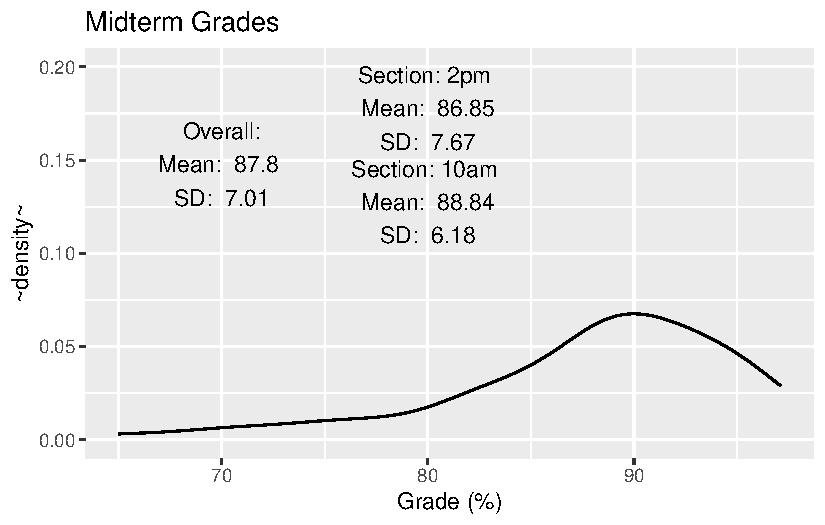
\includegraphics{Lecture12_files/figure-pdf/unnamed-chunk-1-1.pdf}

\subsection{Activity 1: Review your
midterm}\label{activity-1-review-your-midterm}

\begin{itemize}
\item
  Check the page totals (bottom corner) and exam totals (first page)
\item
  Find where you lost the most points. What did you do incorrectly?
\item
  What was something you did well?
\item
  Fill out the canvas Quiz
\end{itemize}

\subsection{R code for SARIMA models}\label{r-code-for-sarima-models}

\begin{itemize}
\tightlist
\item
  \texttt{sarima} function from the \texttt{astsa} package
\item
  \texttt{auto.arima} function from the \texttt{forecast} package
\item
  \texttt{model} function from the \texttt{fable} package
\end{itemize}

Which to use??? They all are fine, but output the model object
differently, so the model output won't work with functions from other
packages.

\subsection{\texorpdfstring{{Example: Trying to use \texttt{sarima}
output with \texttt{fable}
diagnostics}}{Example: Trying to use sarima output with fable diagnostics}}\label{example-trying-to-use-sarima-output-with-fable-diagnostics}

You get an error!

\begin{Shaded}
\begin{Highlighting}[]
\FunctionTok{library}\NormalTok{(fpp3)}
\DocumentationTok{\#\# Registered S3 method overwritten by \textquotesingle{}tsibble\textquotesingle{}:}
\DocumentationTok{\#\#   method               from }
\DocumentationTok{\#\#   as\_tibble.grouped\_df dplyr}
\DocumentationTok{\#\# {-}{-} Attaching packages {-}{-}{-}{-}{-}{-}{-}{-}{-}{-}{-}{-}{-}{-}{-}{-}{-}{-}{-}{-}{-}{-}{-}{-}{-}{-}{-}{-}{-}{-}{-}{-}{-}{-}{-}{-}{-}{-}{-}{-}{-}{-}{-}{-} fpp3 1.0.1 {-}{-}}
\DocumentationTok{\#\# v tsibble     1.1.5     v feasts      0.4.1}
\DocumentationTok{\#\# v tsibbledata 0.4.1     v fable       0.4.0}
\DocumentationTok{\#\# {-}{-} Conflicts {-}{-}{-}{-}{-}{-}{-}{-}{-}{-}{-}{-}{-}{-}{-}{-}{-}{-}{-}{-}{-}{-}{-}{-}{-}{-}{-}{-}{-}{-}{-}{-}{-}{-}{-}{-}{-}{-}{-}{-}{-}{-}{-}{-}{-}{-}{-}{-}{-} fpp3\_conflicts {-}{-}}
\DocumentationTok{\#\# x lubridate::date()    masks base::date()}
\DocumentationTok{\#\# x dplyr::filter()      masks stats::filter()}
\DocumentationTok{\#\# x tsibble::intersect() masks base::intersect()}
\DocumentationTok{\#\# x tsibble::interval()  masks lubridate::interval()}
\DocumentationTok{\#\# x dplyr::lag()         masks stats::lag()}
\DocumentationTok{\#\# x tsibble::setdiff()   masks base::setdiff()}
\DocumentationTok{\#\# x tsibble::union()     masks base::union()}
\FunctionTok{library}\NormalTok{(astsa)}

\NormalTok{log\_gnp }\OtherTok{\textless{}{-}} \FunctionTok{log}\NormalTok{(gnp)}

\NormalTok{sarima\_model }\OtherTok{\textless{}{-}} \FunctionTok{sarima}\NormalTok{(log\_gnp, }\AttributeTok{p =} \DecValTok{1}\NormalTok{, }\AttributeTok{d =} \DecValTok{1}\NormalTok{, }\AttributeTok{q =} \DecValTok{0}\NormalTok{, }\AttributeTok{P =} \DecValTok{0}\NormalTok{, }\AttributeTok{D =} \DecValTok{0}\NormalTok{, }\AttributeTok{Q =} \DecValTok{0}\NormalTok{, }\AttributeTok{details =} \ConstantTok{FALSE}\NormalTok{)}
\DocumentationTok{\#\# \textless{}\textgreater{}\textless{}\textgreater{}\textless{}\textgreater{}\textless{}\textgreater{}\textless{}\textgreater{}\textless{}\textgreater{}\textless{}\textgreater{}\textless{}\textgreater{}\textless{}\textgreater{}\textless{}\textgreater{}\textless{}\textgreater{}\textless{}\textgreater{}\textless{}\textgreater{}\textless{}\textgreater{}}
\DocumentationTok{\#\#  }
\DocumentationTok{\#\# Coefficients: }
\DocumentationTok{\#\#          Estimate     SE t.value p.value}
\DocumentationTok{\#\# ar1        0.3467 0.0627  5.5255       0}
\DocumentationTok{\#\# constant   0.0083 0.0010  8.5398       0}
\DocumentationTok{\#\# }
\DocumentationTok{\#\# sigma\^{}2 estimated as 9.029576e{-}05 on 220 degrees of freedom }
\DocumentationTok{\#\#  }
\DocumentationTok{\#\# AIC = {-}6.446939  AICc = {-}6.446692  BIC = {-}6.400957 }
\DocumentationTok{\#\# }

\NormalTok{diagnostics }\OtherTok{\textless{}{-}}\NormalTok{ sarima\_model }\SpecialCharTok{|\textgreater{}}
  \FunctionTok{residuals}\NormalTok{() }\SpecialCharTok{|\textgreater{}}
  \FunctionTok{ACF}\NormalTok{() }\SpecialCharTok{|\textgreater{}}
  \FunctionTok{gg\_tsdisplay}\NormalTok{()}
\DocumentationTok{\#\# Error in UseMethod("measured\_vars"): no applicable method for \textquotesingle{}measured\_vars\textquotesingle{} applied to an object of class "NULL"}
\end{Highlighting}
\end{Shaded}

\subsection{\texorpdfstring{Example: trying to use \texttt{fable} output
with \texttt{sarima}
diagnostics}{Example: trying to use fable output with sarima diagnostics}}\label{example-trying-to-use-fable-output-with-sarima-diagnostics}

Since \texttt{sarima} outputs diagnostics when you fit the model, you
could just re-fit the model with \texttt{sarima} and then use the
diagnostics.

\begin{Shaded}
\begin{Highlighting}[]
\NormalTok{fable\_model }\OtherTok{\textless{}{-}}\NormalTok{ log\_gnp }\SpecialCharTok{|\textgreater{}} 
  \FunctionTok{as\_tsibble}\NormalTok{() }\SpecialCharTok{|\textgreater{}}
  \FunctionTok{model}\NormalTok{(}\FunctionTok{ARIMA}\NormalTok{(value }\SpecialCharTok{\textasciitilde{}} \FunctionTok{pdq}\NormalTok{(}\DecValTok{1}\NormalTok{,}\DecValTok{1}\NormalTok{,}\DecValTok{0}\NormalTok{) }\SpecialCharTok{+} \FunctionTok{PDQ}\NormalTok{(}\DecValTok{0}\NormalTok{,}\DecValTok{0}\NormalTok{,}\DecValTok{0}\NormalTok{))) }\SpecialCharTok{|\textgreater{}} \FunctionTok{report}\NormalTok{()}
\DocumentationTok{\#\# Series: value }
\DocumentationTok{\#\# Model: ARIMA(1,1,0) w/ drift }
\DocumentationTok{\#\# }
\DocumentationTok{\#\# Coefficients:}
\DocumentationTok{\#\#          ar1  constant}
\DocumentationTok{\#\#       0.3467    0.0054}
\DocumentationTok{\#\# s.e.  0.0627    0.0006}
\DocumentationTok{\#\# }
\DocumentationTok{\#\# sigma\^{}2 estimated as 9.136e{-}05:  log likelihood=718.61}
\DocumentationTok{\#\# AIC={-}1431.22   AICc={-}1431.11   BIC={-}1421.01}

\FunctionTok{sarima}\NormalTok{(fable\_model) }\DocumentationTok{\#\# doesn\textquotesingle{}t work}
\DocumentationTok{\#\# Error in sarima(fable\_model): argument "d" is missing, with no default}
\end{Highlighting}
\end{Shaded}

\begin{Shaded}
\begin{Highlighting}[]
\DocumentationTok{\#\# fit the same model, but with default details = TRUE.}
\FunctionTok{sarima}\NormalTok{(log\_gnp, }\AttributeTok{p =} \DecValTok{1}\NormalTok{, }\AttributeTok{d =} \DecValTok{1}\NormalTok{, }\AttributeTok{q =} \DecValTok{0}\NormalTok{, }\AttributeTok{P =} \DecValTok{0}\NormalTok{, }\AttributeTok{D =} \DecValTok{0}\NormalTok{, }\AttributeTok{Q =} \DecValTok{0}\NormalTok{)}
\end{Highlighting}
\end{Shaded}

\begin{verbatim}
initial  value -4.589567 
iter   2 value -4.654150
iter   3 value -4.654150
iter   4 value -4.654151
iter   4 value -4.654151
iter   4 value -4.654151
final  value -4.654151 
converged
initial  value -4.655919 
iter   2 value -4.655921
iter   3 value -4.655921
iter   4 value -4.655922
iter   5 value -4.655922
iter   5 value -4.655922
iter   5 value -4.655922
final  value -4.655922 
converged
<><><><><><><><><><><><><><>
 
Coefficients: 
         Estimate     SE t.value p.value
ar1        0.3467 0.0627  5.5255       0
constant   0.0083 0.0010  8.5398       0

sigma^2 estimated as 9.029576e-05 on 220 degrees of freedom 
 
AIC = -6.446939  AICc = -6.446692  BIC = -6.400957 
 
\end{verbatim}

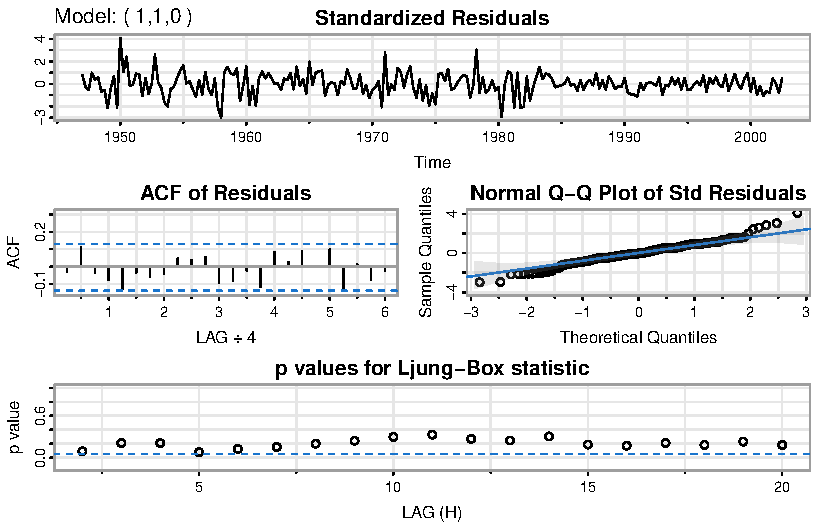
\includegraphics{Lecture12_files/figure-pdf/unnamed-chunk-4-1.pdf}

\subsection{Activity 2: Putting it all
together}\label{activity-2-putting-it-all-together}

\begin{itemize}
\tightlist
\item
  Download ``ARIMA code cheat sheet.docx'' from Canvas
\item
  Pick one column
\item
  Fill in the blanks with the correct functions
\end{itemize}

\subsection{Forecasting}\label{forecasting}

Given the data and a model that fits the data, we want to predict future
values

How can we do this - by ``hand'' (or just ``manually'' using code) -
using \texttt{fable} or \texttt{astsa} functions

Also, how do we plot these forecasts?

\subsection{\texorpdfstring{{Forecasting using \texttt{fable} or
\texttt{astsa}
functions}}{Forecasting using fable or astsa functions}}\label{forecasting-using-fable-or-astsa-functions}

\texttt{fable} functions

\begin{enumerate}
\def\labelenumi{\arabic{enumi}.}
\item
  Fit model using \texttt{model()} and \texttt{ARIMA()}
\item
  Forecast using \texttt{forecast()} specifying \texttt{h}
\end{enumerate}

\begin{Shaded}
\begin{Highlighting}[]
\NormalTok{fit }\OtherTok{\textless{}{-}}\NormalTok{ log\_gnp }\SpecialCharTok{|\textgreater{}} 
  \FunctionTok{as\_tsibble}\NormalTok{() }\SpecialCharTok{|\textgreater{}}
  \FunctionTok{model}\NormalTok{(}\FunctionTok{ARIMA}\NormalTok{(value }\SpecialCharTok{\textasciitilde{}} \FunctionTok{pdq}\NormalTok{(}\DecValTok{1}\NormalTok{,}\DecValTok{1}\NormalTok{,}\DecValTok{0}\NormalTok{) }\SpecialCharTok{+} \FunctionTok{PDQ}\NormalTok{(}\DecValTok{0}\NormalTok{,}\DecValTok{0}\NormalTok{,}\DecValTok{0}\NormalTok{))) }\DocumentationTok{\#\# force nonseasonal}

\NormalTok{fit }\SpecialCharTok{|\textgreater{}} \FunctionTok{forecast}\NormalTok{(}\AttributeTok{h =} \DecValTok{10}\NormalTok{)}
\end{Highlighting}
\end{Shaded}

\begin{verbatim}
# A fable: 10 x 4 [1Q]
# Key:     .model [1]
   .model                                       index
   <chr>                                        <qtr>
 1 ARIMA(value ~ pdq(1, 1, 0) + PDQ(0, 0, 0)) 2002 Q4
 2 ARIMA(value ~ pdq(1, 1, 0) + PDQ(0, 0, 0)) 2003 Q1
 3 ARIMA(value ~ pdq(1, 1, 0) + PDQ(0, 0, 0)) 2003 Q2
 4 ARIMA(value ~ pdq(1, 1, 0) + PDQ(0, 0, 0)) 2003 Q3
 5 ARIMA(value ~ pdq(1, 1, 0) + PDQ(0, 0, 0)) 2003 Q4
 6 ARIMA(value ~ pdq(1, 1, 0) + PDQ(0, 0, 0)) 2004 Q1
 7 ARIMA(value ~ pdq(1, 1, 0) + PDQ(0, 0, 0)) 2004 Q2
 8 ARIMA(value ~ pdq(1, 1, 0) + PDQ(0, 0, 0)) 2004 Q3
 9 ARIMA(value ~ pdq(1, 1, 0) + PDQ(0, 0, 0)) 2004 Q4
10 ARIMA(value ~ pdq(1, 1, 0) + PDQ(0, 0, 0)) 2005 Q1
# i 2 more variables: value <dist>, .mean <dbl>
\end{verbatim}

\begin{itemize}
\item
  \texttt{astsa} functions

  \begin{enumerate}
  \def\labelenumi{\arabic{enumi}.}
  \tightlist
  \item
    Determine model order using acf/pacf, check model fit using
    \texttt{sarima}
  \item
    Use \texttt{sarima.for} to forecast (with order you chose-- re-fits
    model)
  \end{enumerate}
\end{itemize}

\begin{Shaded}
\begin{Highlighting}[]
\NormalTok{sarima\_model }\OtherTok{\textless{}{-}} \FunctionTok{sarima}\NormalTok{(log\_gnp, }\AttributeTok{p =} \DecValTok{1}\NormalTok{, }\AttributeTok{d =} \DecValTok{1}\NormalTok{, }\AttributeTok{q =} \DecValTok{0}\NormalTok{, }\AttributeTok{P =} \DecValTok{0}\NormalTok{, }\AttributeTok{D =} \DecValTok{0}\NormalTok{, }\AttributeTok{Q =} \DecValTok{0}\NormalTok{)}
\end{Highlighting}
\end{Shaded}

\begin{verbatim}
initial  value -4.589567 
iter   2 value -4.654150
iter   3 value -4.654150
iter   4 value -4.654151
iter   4 value -4.654151
iter   4 value -4.654151
final  value -4.654151 
converged
initial  value -4.655919 
iter   2 value -4.655921
iter   3 value -4.655921
iter   4 value -4.655922
iter   5 value -4.655922
iter   5 value -4.655922
iter   5 value -4.655922
final  value -4.655922 
converged
<><><><><><><><><><><><><><>
 
Coefficients: 
         Estimate     SE t.value p.value
ar1        0.3467 0.0627  5.5255       0
constant   0.0083 0.0010  8.5398       0

sigma^2 estimated as 9.029576e-05 on 220 degrees of freedom 
 
AIC = -6.446939  AICc = -6.446692  BIC = -6.400957 
 
\end{verbatim}

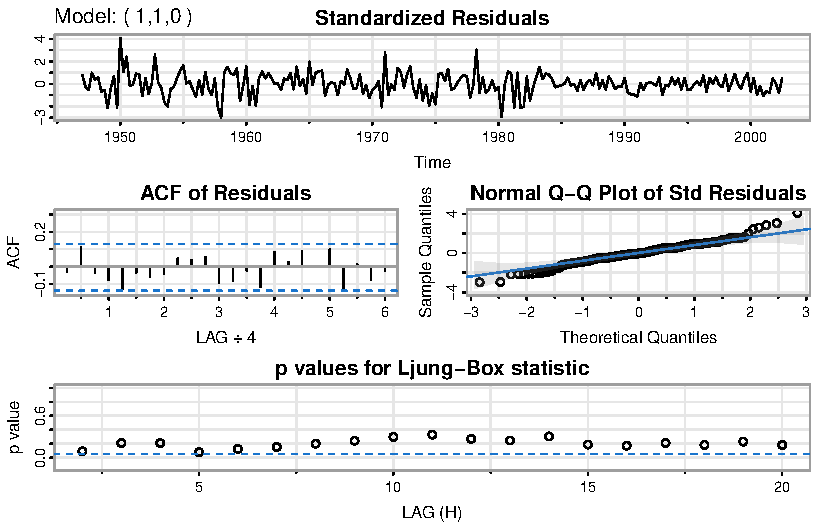
\includegraphics{Lecture12_files/figure-pdf/unnamed-chunk-6-1.pdf}

\begin{Shaded}
\begin{Highlighting}[]
\FunctionTok{sarima.for}\NormalTok{(log\_gnp,}\AttributeTok{p =} \DecValTok{1}\NormalTok{, }\AttributeTok{d =} \DecValTok{1}\NormalTok{, }\AttributeTok{q =} \DecValTok{0}\NormalTok{, }\AttributeTok{P =} \DecValTok{0}\NormalTok{, }\AttributeTok{D =} \DecValTok{0}\NormalTok{, }\AttributeTok{Q =} \DecValTok{0}\NormalTok{, }\AttributeTok{n.ahead =} \DecValTok{10}\NormalTok{, }\AttributeTok{plot =}\NormalTok{ F)}
\end{Highlighting}
\end{Shaded}

\begin{verbatim}
$pred
         Qtr1     Qtr2     Qtr3     Qtr4
2002                            9.165886
2003 9.174510 9.182946 9.191316 9.199664
2004 9.208004 9.216342 9.224678 9.233014
2005 9.241350                           

$se
            Qtr1        Qtr2        Qtr3        Qtr4
2002                                     0.009502408
2003 0.015938787 0.021173624 0.025569341 0.029380482
2004 0.032772142 0.035850982 0.038687708 0.041330887
2005 0.043815131                                    
\end{verbatim}

\subsection{Compare predictions}\label{compare-predictions}

Yay! They're the same :)

\begin{Shaded}
\begin{Highlighting}[]
\NormalTok{fable\_forecast }\OtherTok{\textless{}{-}}\NormalTok{ fit }\SpecialCharTok{|\textgreater{}} \FunctionTok{forecast}\NormalTok{(}\AttributeTok{h =} \DecValTok{10}\NormalTok{)}
\NormalTok{astsa\_forecast }\OtherTok{\textless{}{-}} \FunctionTok{sarima.for}\NormalTok{(log\_gnp,}\AttributeTok{p =} \DecValTok{1}\NormalTok{, }\AttributeTok{d =} \DecValTok{1}\NormalTok{, }\AttributeTok{q =} \DecValTok{0}\NormalTok{, }\AttributeTok{P =} \DecValTok{0}\NormalTok{, }\AttributeTok{D =} \DecValTok{0}\NormalTok{, }\AttributeTok{Q =} \DecValTok{0}\NormalTok{, }\AttributeTok{n.ahead =} \DecValTok{10}\NormalTok{, }\AttributeTok{plot =}\NormalTok{ F)}

\FunctionTok{cbind}\NormalTok{(fable\_forecast}\SpecialCharTok{$}\NormalTok{.mean,astsa\_forecast}\SpecialCharTok{$}\NormalTok{pred)}
\end{Highlighting}
\end{Shaded}

\begin{verbatim}
        fable_forecast$.mean astsa_forecast$pred
2002 Q4             9.165886            9.165886
2003 Q1             9.174510            9.174510
2003 Q2             9.182946            9.182946
2003 Q3             9.191316            9.191316
2003 Q4             9.199664            9.199664
2004 Q1             9.208004            9.208004
2004 Q2             9.216342            9.216342
2004 Q3             9.224678            9.224678
2004 Q4             9.233014            9.233014
2005 Q1             9.241350            9.241350
\end{verbatim}

\subsection{\texorpdfstring{Plot the forecast
(\texttt{fable})}{Plot the forecast (fable)}}\label{plot-the-forecast-fable}

\begin{Shaded}
\begin{Highlighting}[]
\NormalTok{fable\_forecast }\SpecialCharTok{|\textgreater{}} \FunctionTok{autoplot}\NormalTok{(log\_gnp)}
\end{Highlighting}
\end{Shaded}

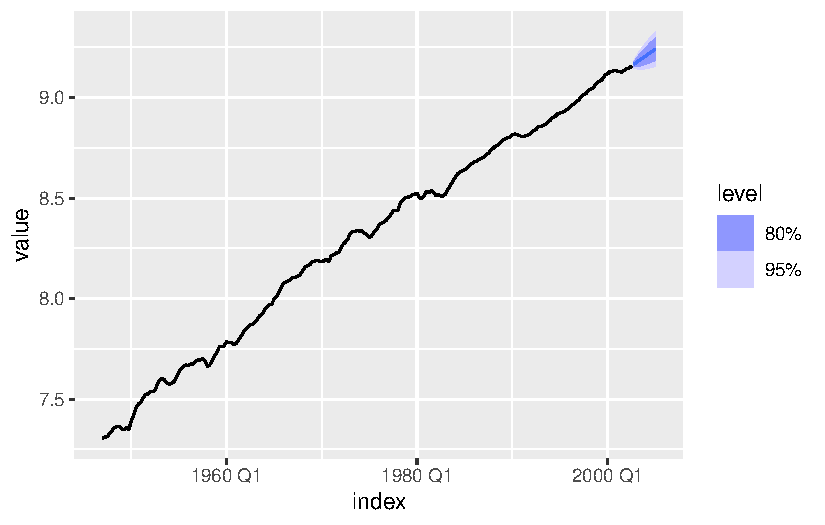
\includegraphics{Lecture12_files/figure-pdf/unnamed-chunk-8-1.pdf}

\subsection{\texorpdfstring{Plot the forecast
(\texttt{astsa})}{Plot the forecast (astsa)}}\label{plot-the-forecast-astsa}

\begin{Shaded}
\begin{Highlighting}[]
\FunctionTok{sarima.for}\NormalTok{(log\_gnp,}\AttributeTok{p =} \DecValTok{1}\NormalTok{, }\AttributeTok{d =} \DecValTok{1}\NormalTok{, }\AttributeTok{q =} \DecValTok{0}\NormalTok{, }\AttributeTok{P =} \DecValTok{0}\NormalTok{, }\AttributeTok{D =} \DecValTok{0}\NormalTok{, }\AttributeTok{Q =} \DecValTok{0}\NormalTok{, }\AttributeTok{n.ahead =} \DecValTok{10}\NormalTok{, }\AttributeTok{plot =}\NormalTok{ T)}
\end{Highlighting}
\end{Shaded}

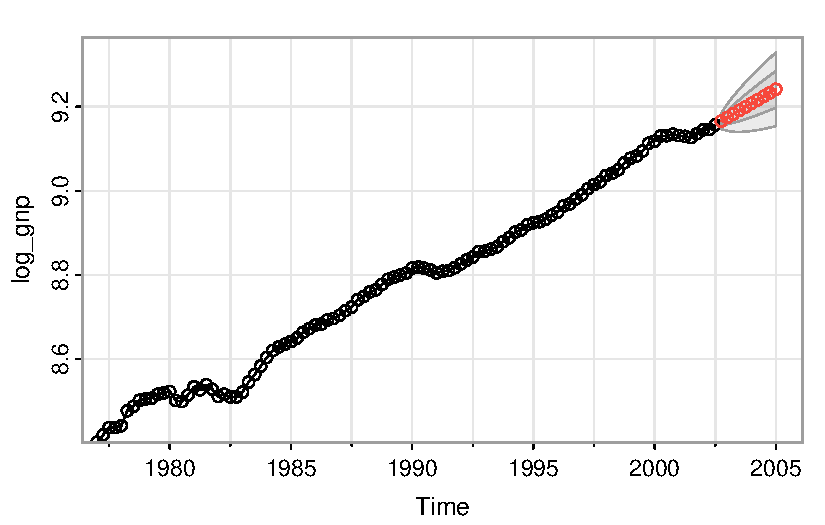
\includegraphics{Lecture12_files/figure-pdf/unnamed-chunk-9-1.pdf}

\begin{verbatim}
$pred
         Qtr1     Qtr2     Qtr3     Qtr4
2002                            9.165886
2003 9.174510 9.182946 9.191316 9.199664
2004 9.208004 9.216342 9.224678 9.233014
2005 9.241350                           

$se
            Qtr1        Qtr2        Qtr3        Qtr4
2002                                     0.009502408
2003 0.015938787 0.021173624 0.025569341 0.029380482
2004 0.032772142 0.035850982 0.038687708 0.041330887
2005 0.043815131                                    
\end{verbatim}

\subsection{Forecasting ``by hand''}\label{forecasting-by-hand}

\begin{enumerate}
\def\labelenumi{\arabic{enumi}.}
\tightlist
\item
  Write down the equation of your model based on the output
\item
  Get the observations you need to populate the forecast
\item
  Calculate the forecast, pushing forward your next forecasted value
  through the equation
\end{enumerate}

\subsection{Forecasting ``by hand''}\label{forecasting-by-hand-1}

\begin{Shaded}
\begin{Highlighting}[]
\NormalTok{astsa\_model }\OtherTok{\textless{}{-}} \FunctionTok{sarima}\NormalTok{(log\_gnp, }\AttributeTok{p =} \DecValTok{1}\NormalTok{, }\AttributeTok{d =} \DecValTok{1}\NormalTok{, }\AttributeTok{q =} \DecValTok{0}\NormalTok{, }\AttributeTok{P =} \DecValTok{0}\NormalTok{, }\AttributeTok{D =} \DecValTok{0}\NormalTok{, }\AttributeTok{Q =} \DecValTok{0}\NormalTok{, }\AttributeTok{details =} \ConstantTok{FALSE}\NormalTok{)}
\end{Highlighting}
\end{Shaded}

\begin{verbatim}
<><><><><><><><><><><><><><>
 
Coefficients: 
         Estimate     SE t.value p.value
ar1        0.3467 0.0627  5.5255       0
constant   0.0083 0.0010  8.5398       0

sigma^2 estimated as 9.029576e-05 on 220 degrees of freedom 
 
AIC = -6.446939  AICc = -6.446692  BIC = -6.400957 
 
\end{verbatim}

(apparent) \texttt{fable} forecast equation:
\(\hat{x_t} = 0.0054 + 0.3467\cdot x_{t-1}\)

(apparent) \texttt{astsa} forecast equation:
\(\hat{x_t} = 0.0083 + 0.3467\cdot x_{t-1}\)

\subsection{Activity: Forecasting ``by
hand''}\label{activity-forecasting-by-hand}

\texttt{fable} forecast equation:
\(\hat{x_t} = 0.0054 + 0.3467\cdot x_{t-1}\)

\texttt{astsa} forecast equation:
\(\hat{x_t} = 0.0083 + 0.3467\cdot x_{t-1}\)

\subsection{Activity Solution: Forecasting ``by
hand''}\label{activity-solution-forecasting-by-hand}

\begin{Shaded}
\begin{Highlighting}[]
\FunctionTok{data.frame}\NormalTok{(}\AttributeTok{time =} \FunctionTok{tail}\NormalTok{(}\FunctionTok{time}\NormalTok{(log\_gnp)), }\AttributeTok{log\_gnp =} \FunctionTok{tail}\NormalTok{(log\_gnp), }\AttributeTok{diff\_log\_gnp =} \FunctionTok{tail}\NormalTok{(}\FunctionTok{diff}\NormalTok{(log\_gnp)))}
\end{Highlighting}
\end{Shaded}

\begin{verbatim}
     time  log_gnp  diff_log_gnp
1 2001.25 9.129597 -0.0018845451
2 2001.50 9.126937 -0.0026595616
3 2001.75 9.135994  0.0090568862
4 2002.00 9.145002  0.0090076208
5 2002.25 9.145983  0.0009816371
6 2002.50 9.156718  0.0107348840
\end{verbatim}

\texttt{fable} forecast equation:
\(\hat{x_t} = 0.0054 + 0.3467\cdot x_{t-1}\)

\begin{itemize}
\tightlist
\item
  \(\hat{x}_{2002 Q4} = 0.0054 + 0.3467\cdot x_{2002 Q3} = 0.0054 + 0.3467\cdot 9.156718 = 3.1800034\)
\end{itemize}

\texttt{astsa} forecast equation:
\(\hat{x_t} = 0.0083 + 0.3467\cdot x_{t-1}\)

\begin{itemize}
\tightlist
\item
  \(\hat{x}_{2002 Q4} = 0.0083 + 0.3467\cdot x_{2002 Q3} = 0.0083 + 0.3467\cdot 9.156718 = 3.182934\)
\end{itemize}

These values don't make sense, and don't match?

\subsection{Reconciling the by hand
difference}\label{reconciling-the-by-hand-difference}

For our AR(1) model, we have

\[
(1 - \phi B)(1-B)y_t = c + error
\] Ignoring the error since we want a forecast of the mean, applying the
backwards shift operator, F.O.I.L., using our estimate of \(\phi\), and
solving for \(y_t\) we get:

\[
\hat{x}_t = x_{t-1} + \hat{\phi}(x_{t-1} - x_{t-2}))+ c
\]

\subsection{Let's try this equation!}\label{lets-try-this-equation}

\[
\hat{x}_{2002 Q4} = x_{2002 Q3} + \hat{\phi}(x_{2002 Q3} - x_{2002 Q2}))+ c
\]

\begin{Shaded}
\begin{Highlighting}[]
\DocumentationTok{\#\# for fable}
\FloatTok{9.156718} \SpecialCharTok{+} \FloatTok{0.3467}\SpecialCharTok{*}\NormalTok{(}\FloatTok{9.156718} \SpecialCharTok{{-}} \FloatTok{9.145983}\NormalTok{) }\SpecialCharTok{+} \FloatTok{0.0054}
\end{Highlighting}
\end{Shaded}

\begin{verbatim}
[1] 9.16584
\end{verbatim}

\begin{Shaded}
\begin{Highlighting}[]
\DocumentationTok{\#\# for sarima}
\FloatTok{9.156718} \SpecialCharTok{+} \FloatTok{0.3467}\SpecialCharTok{*}\NormalTok{(}\FloatTok{9.156718} \SpecialCharTok{{-}} \FloatTok{9.145983}\NormalTok{) }\SpecialCharTok{+} \FloatTok{0.0083}
\end{Highlighting}
\end{Shaded}

\begin{verbatim}
[1] 9.16874
\end{verbatim}

That's better, but only \texttt{fable} matches the forecast functions?

\subsection{Comparing constants}\label{comparing-constants}

Takeaway: Different packages estimate the ``constant'' differently!

See https://otexts.com/fpp3/arima-r.html\#understanding-constants-in-r.

\begin{Shaded}
\begin{Highlighting}[]
\FunctionTok{library}\NormalTok{(fpp3)}
\FunctionTok{library}\NormalTok{(astsa)}
\NormalTok{log\_gnp }\OtherTok{\textless{}{-}} \FunctionTok{log}\NormalTok{(gnp)}

\NormalTok{fable\_model }\OtherTok{\textless{}{-}}\NormalTok{ log\_gnp }\SpecialCharTok{|\textgreater{}} 
  \FunctionTok{as\_tsibble}\NormalTok{() }\SpecialCharTok{|\textgreater{}}
  \FunctionTok{model}\NormalTok{(}\FunctionTok{ARIMA}\NormalTok{(value }\SpecialCharTok{\textasciitilde{}} \FunctionTok{pdq}\NormalTok{(}\DecValTok{1}\NormalTok{,}\DecValTok{1}\NormalTok{,}\DecValTok{0}\NormalTok{) }\SpecialCharTok{+} \FunctionTok{PDQ}\NormalTok{(}\DecValTok{0}\NormalTok{,}\DecValTok{0}\NormalTok{,}\DecValTok{0}\NormalTok{))) }\DocumentationTok{\#\# force nonseasonal}

\NormalTok{fable\_model }\SpecialCharTok{|\textgreater{}} \FunctionTok{report}\NormalTok{()}
\DocumentationTok{\#\# Series: value }
\DocumentationTok{\#\# Model: ARIMA(1,1,0) w/ drift }
\DocumentationTok{\#\# }
\DocumentationTok{\#\# Coefficients:}
\DocumentationTok{\#\#          ar1  constant}
\DocumentationTok{\#\#       0.3467    0.0054}
\DocumentationTok{\#\# s.e.  0.0627    0.0006}
\DocumentationTok{\#\# }
\DocumentationTok{\#\# sigma\^{}2 estimated as 9.136e{-}05:  log likelihood=718.61}
\DocumentationTok{\#\# AIC={-}1431.22   AICc={-}1431.11   BIC={-}1421.01}
\NormalTok{sarima\_model }\OtherTok{\textless{}{-}} \FunctionTok{sarima}\NormalTok{(log\_gnp, }\AttributeTok{p =} \DecValTok{1}\NormalTok{, }\AttributeTok{d =} \DecValTok{1}\NormalTok{, }\AttributeTok{q =} \DecValTok{0}\NormalTok{, }\AttributeTok{P =} \DecValTok{0}\NormalTok{, }\AttributeTok{D =} \DecValTok{0}\NormalTok{, }\AttributeTok{Q =} \DecValTok{0}\NormalTok{, }\AttributeTok{details =}\NormalTok{ F)}
\DocumentationTok{\#\# \textless{}\textgreater{}\textless{}\textgreater{}\textless{}\textgreater{}\textless{}\textgreater{}\textless{}\textgreater{}\textless{}\textgreater{}\textless{}\textgreater{}\textless{}\textgreater{}\textless{}\textgreater{}\textless{}\textgreater{}\textless{}\textgreater{}\textless{}\textgreater{}\textless{}\textgreater{}\textless{}\textgreater{}}
\DocumentationTok{\#\#  }
\DocumentationTok{\#\# Coefficients: }
\DocumentationTok{\#\#          Estimate     SE t.value p.value}
\DocumentationTok{\#\# ar1        0.3467 0.0627  5.5255       0}
\DocumentationTok{\#\# constant   0.0083 0.0010  8.5398       0}
\DocumentationTok{\#\# }
\DocumentationTok{\#\# sigma\^{}2 estimated as 9.029576e{-}05 on 220 degrees of freedom }
\DocumentationTok{\#\#  }
\DocumentationTok{\#\# AIC = {-}6.446939  AICc = {-}6.446692  BIC = {-}6.400957 }
\DocumentationTok{\#\# }

\NormalTok{mu }\OtherTok{=} \FunctionTok{mean}\NormalTok{(}\FunctionTok{diff}\NormalTok{(log\_gnp))}

\NormalTok{mu}\SpecialCharTok{*}\NormalTok{(}\DecValTok{1}\SpecialCharTok{{-}}\NormalTok{sarima\_model}\SpecialCharTok{$}\NormalTok{fit}\SpecialCharTok{$}\NormalTok{coef[}\DecValTok{1}\NormalTok{])}
\DocumentationTok{\#\#         ar1 }
\DocumentationTok{\#\# 0.005447277}
\end{Highlighting}
\end{Shaded}

\subsection{Actual by-hand forecast
equations:}\label{actual-by-hand-forecast-equations}

For \texttt{fable}, where \(c\) is the constant outputted. \[
\hat{x}_{2002 Q4} = x_{2002 Q3} + \hat{\phi}(x_{2002 Q3} - x_{2002 Q2}))+ c_{fable}
\]

For \texttt{astsa}, where \(c\) is the constant outputted. \[
\hat{x}_{2002 Q4} = x_{2002 Q3} + \phi(x_{2002 Q3} - x_{2002 Q2}))+ mean(diff(x_t))(1 - \hat{\phi})
\]

\begin{Shaded}
\begin{Highlighting}[]
\DocumentationTok{\#\# for astsa}

\FloatTok{9.156718} \SpecialCharTok{+} \FloatTok{0.3467}\SpecialCharTok{*}\NormalTok{(}\FloatTok{9.156718} \SpecialCharTok{{-}} \FloatTok{9.145983}\NormalTok{) }\SpecialCharTok{+} \FunctionTok{mean}\NormalTok{(}\FunctionTok{diff}\NormalTok{(log\_gnp))}\SpecialCharTok{*}\NormalTok{(}\DecValTok{1}\SpecialCharTok{{-}} \FloatTok{0.3467}\NormalTok{) }
\end{Highlighting}
\end{Shaded}

\begin{verbatim}
[1] 9.165887
\end{verbatim}

\subsection{More on the Ljung-box
statistic}\label{more-on-the-ljung-box-statistic}

\begin{itemize}
\tightlist
\item
  ``another way to view the ACF of the residuals''
\item
  ``not a bunch of highly dependent tests''
\item
  ``accumulation of autocorrelation''
\item
  ``considers the magnitudes'' of the autocorrelations all together
\end{itemize}

\[
Q = n(n+2) + \sum_{h=1}^H \frac{\hat{\rho}_{resid}(h)^2}{n-h}
\] Test statistic used to calcualte p-values in the \texttt{sarima}
output-- the \(\hat{\rho}_{resid}(h)\) is the sample acf we plot using
\texttt{acf} or \texttt{acf1}.

\subsection{ETS Models}\label{ets-models}

Stepping away from ARIMA for the time being\ldots{}

\subsection{Smoothing}\label{smoothing}

We have seen several smoothers:

\begin{itemize}
\tightlist
\item
  Moving Average
\item
  Loess
\item
  Kernel
\end{itemize}

We have also seen the \texttt{decompose} function, but emphasized it is
an exploratory data analysis tool.

What if we wanted to use these equations for forecasting?

\subsection{Simple exponential
smoothing}\label{simple-exponential-smoothing}

\begin{itemize}
\item
  useful for forecasting data with no trend or seasonal component
\item
  Predicts the future as a weighted average of the past, where the
  weights decrease exponentially the further back in time you go
\end{itemize}

\subsection{Example: Algerian Exports (FPP
8.1)}\label{example-algerian-exports-fpp-8.1}

\begin{Shaded}
\begin{Highlighting}[]
\NormalTok{algeria\_economy }\OtherTok{\textless{}{-}}\NormalTok{ global\_economy }\SpecialCharTok{|\textgreater{}}
  \FunctionTok{filter}\NormalTok{(Country }\SpecialCharTok{==} \StringTok{"Algeria"}\NormalTok{)}
\NormalTok{algeria\_economy }\SpecialCharTok{|\textgreater{}}
  \FunctionTok{autoplot}\NormalTok{(Exports) }\SpecialCharTok{+}
  \FunctionTok{labs}\NormalTok{(}\AttributeTok{y =} \StringTok{"\% of GDP"}\NormalTok{, }\AttributeTok{title =} \StringTok{"Exports: Algeria"}\NormalTok{)}
\end{Highlighting}
\end{Shaded}

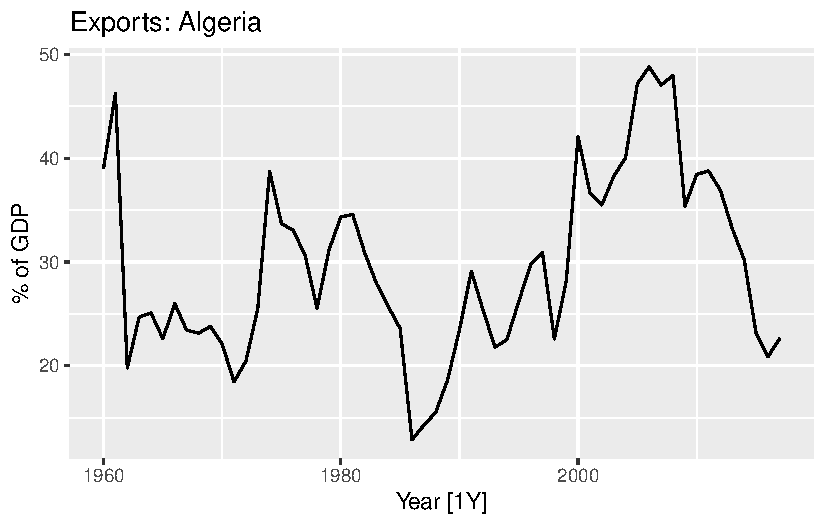
\includegraphics{Lecture12_files/figure-pdf/unnamed-chunk-15-1.pdf}

\subsection{We want a forecast equation\ldots{} here it
is}\label{we-want-a-forecast-equation-here-it-is}

\[
\begin{equation}
  \hat{y}_{T+1|T} = \alpha y_T + \alpha(1-\alpha) y_{T-1} + \alpha(1-\alpha)^2 y_{T-2}+ \cdots,   \tag{8.1}
\end{equation}
\]

\begin{itemize}
\tightlist
\item
  \(\alpha\) is the smoothing parameter
\item
  the weights are the coefficients in front of the \(y_{T-h}\) terms.
\end{itemize}

\subsection{Forecast equation (weighted average
form)}\label{forecast-equation-weighted-average-form}

We can rewrite the equation as:

\[
\hat{y}_{T+1|T} = \alpha y_T + (1-\alpha) \hat{y}_{T|T-1},
\] In order to forecast the next point, we need to just keep track of
the data for the last time point, and the forecast for the last time
point.

Easy to update as new data comes in!

\subsection{Forecast equation (component
form)}\label{forecast-equation-component-form}

More notation, but essentially the same thing as the last slide. This
representation will be helpful later on.

\[
\begin{align*}
  \text{Forecast equation}  && \hat{y}_{t+h|t} & = \ell_{t}\\
  \text{Smoothing equation} && \ell_{t}        & = \alpha y_{t} + (1 - \alpha)\ell_{t-1},
\end{align*}
\]

\subsection{\texorpdfstring{Fitting simple exponential smoothing in
\texttt{fable}}{Fitting simple exponential smoothing in fable}}\label{fitting-simple-exponential-smoothing-in-fable}

A is for additive, N is for none (we'll cover this more next time)

\begin{Shaded}
\begin{Highlighting}[]
\NormalTok{fit }\OtherTok{\textless{}{-}}\NormalTok{ algeria\_economy }\SpecialCharTok{|\textgreater{}}
  \FunctionTok{model}\NormalTok{(}\FunctionTok{ETS}\NormalTok{(Exports }\SpecialCharTok{\textasciitilde{}} \FunctionTok{error}\NormalTok{(}\StringTok{"A"}\NormalTok{) }\SpecialCharTok{+} \FunctionTok{trend}\NormalTok{(}\StringTok{"N"}\NormalTok{) }\SpecialCharTok{+} \FunctionTok{season}\NormalTok{(}\StringTok{"N"}\NormalTok{)))}

\FunctionTok{report}\NormalTok{(fit)}
\end{Highlighting}
\end{Shaded}

\begin{verbatim}
Series: Exports 
Model: ETS(A,N,N) 
  Smoothing parameters:
    alpha = 0.8399875 

  Initial states:
   l[0]
 39.539

  sigma^2:  35.6301

     AIC     AICc      BIC 
446.7154 447.1599 452.8968 
\end{verbatim}

\begin{Shaded}
\begin{Highlighting}[]
\NormalTok{fc }\OtherTok{\textless{}{-}}\NormalTok{ fit }\SpecialCharTok{|\textgreater{}}
  \FunctionTok{forecast}\NormalTok{(}\AttributeTok{h =} \DecValTok{1}\NormalTok{)}
\end{Highlighting}
\end{Shaded}

\subsection{Plot the forecast}\label{plot-the-forecast}

\begin{itemize}
\item
  Note the ``flat'' forecast (because of no trend/seasonal assumption)
\item
  Where did the uncertainty estimates come from??
\end{itemize}

\begin{Shaded}
\begin{Highlighting}[]
\NormalTok{fc }\SpecialCharTok{|\textgreater{}}
  \FunctionTok{autoplot}\NormalTok{(algeria\_economy) }\SpecialCharTok{+}
  \FunctionTok{geom\_line}\NormalTok{(}\FunctionTok{aes}\NormalTok{(}\AttributeTok{y =}\NormalTok{ .fitted), }\AttributeTok{col=}\StringTok{"\#D55E00"}\NormalTok{,}
            \AttributeTok{data =} \FunctionTok{augment}\NormalTok{(fit)) }\SpecialCharTok{+}
  \FunctionTok{labs}\NormalTok{(}\AttributeTok{y=}\StringTok{"\% of GDP"}\NormalTok{, }\AttributeTok{title=}\StringTok{"Exports: Algeria"}\NormalTok{) }\SpecialCharTok{+}
  \FunctionTok{guides}\NormalTok{(}\AttributeTok{colour =} \StringTok{"none"}\NormalTok{)}
\end{Highlighting}
\end{Shaded}

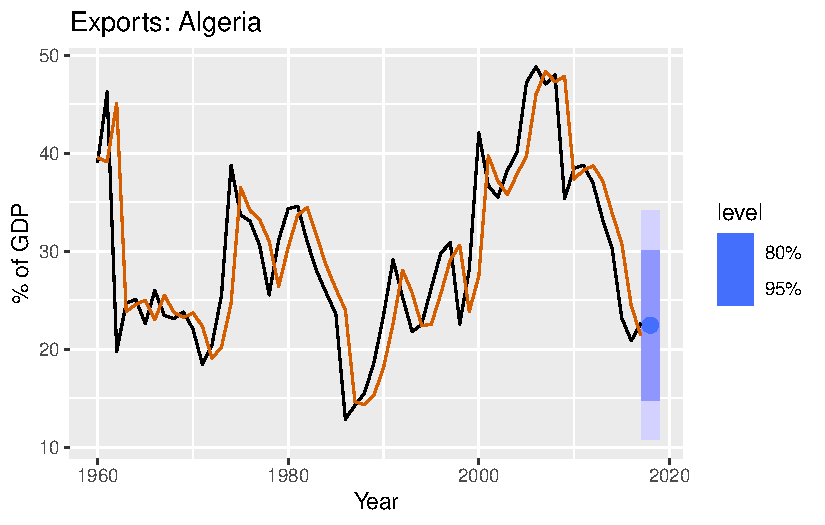
\includegraphics{Lecture12_files/figure-pdf/unnamed-chunk-17-1.pdf}

\subsection{Next time: Holt's Linear
Method}\label{next-time-holts-linear-method}

\begin{itemize}
\tightlist
\item
  forecast data with a trend
\item
  involves three equations: forecast, level, and trend
\end{itemize}

\[
\begin{aligned}
  \text{Forecast equation}&& \hat{y}_{t+h|t} &= \ell_{t} + hb_{t} \\
  \text{Level equation}   && \ell_{t} &= \alpha y_{t} + (1 - \alpha)(\ell_{t-1} + b_{t-1})\\
  \text{Trend equation}   && b_{t}    &= \beta^*(\ell_{t} - \ell_{t-1}) + (1 -\beta^*)b_{t-1},
\end{aligned}
\]

\subsection{Example: Australian Population (FPP
8.2)}\label{example-australian-population-fpp-8.2}

\begin{Shaded}
\begin{Highlighting}[]
\NormalTok{aus\_economy }\OtherTok{\textless{}{-}}\NormalTok{ global\_economy }\SpecialCharTok{|\textgreater{}}
  \FunctionTok{filter}\NormalTok{(Code }\SpecialCharTok{==} \StringTok{"AUS"}\NormalTok{) }\SpecialCharTok{|\textgreater{}}
  \FunctionTok{mutate}\NormalTok{(}\AttributeTok{Pop =}\NormalTok{ Population }\SpecialCharTok{/} \FloatTok{1e6}\NormalTok{)}
\FunctionTok{autoplot}\NormalTok{(aus\_economy, Pop) }\SpecialCharTok{+}
  \FunctionTok{labs}\NormalTok{(}\AttributeTok{y =} \StringTok{"Millions"}\NormalTok{, }\AttributeTok{title =} \StringTok{"Australian population"}\NormalTok{)}
\end{Highlighting}
\end{Shaded}

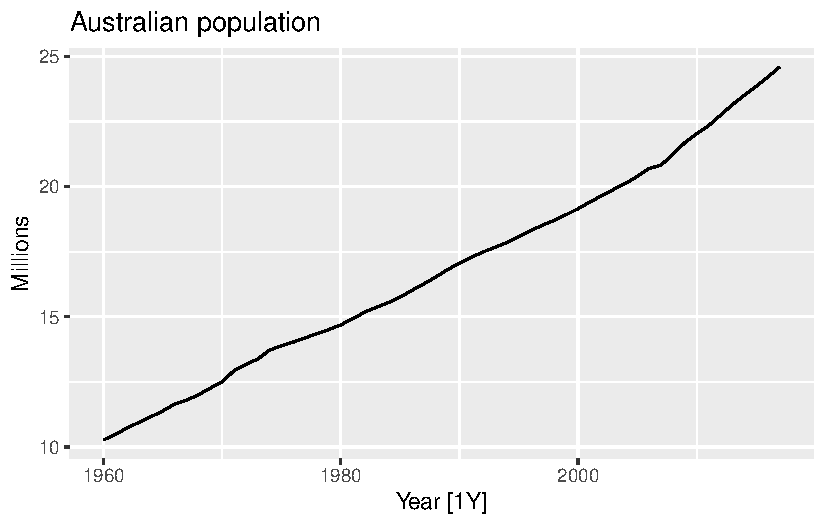
\includegraphics{Lecture12_files/figure-pdf/unnamed-chunk-18-1.pdf}

\subsection{Example: Australian Population (FPP
8.2)}\label{example-australian-population-fpp-8.2-1}

Fit the Holt Linear Method (exponential smoothing w/trend)

\begin{Shaded}
\begin{Highlighting}[]
\NormalTok{fit }\OtherTok{\textless{}{-}}\NormalTok{ aus\_economy }\SpecialCharTok{|\textgreater{}}
  \FunctionTok{model}\NormalTok{(}
    \AttributeTok{AAN =} \FunctionTok{ETS}\NormalTok{(Pop }\SpecialCharTok{\textasciitilde{}} \FunctionTok{error}\NormalTok{(}\StringTok{"A"}\NormalTok{) }\SpecialCharTok{+} \FunctionTok{trend}\NormalTok{(}\StringTok{"A"}\NormalTok{) }\SpecialCharTok{+} \FunctionTok{season}\NormalTok{(}\StringTok{"N"}\NormalTok{))}
\NormalTok{  )}
\NormalTok{fc }\OtherTok{\textless{}{-}}\NormalTok{ fit }\SpecialCharTok{|\textgreater{}} \FunctionTok{forecast}\NormalTok{(}\AttributeTok{h =} \DecValTok{10}\NormalTok{)}
\end{Highlighting}
\end{Shaded}





\end{document}
